% ============================================================================
% BATTERY MANAGEMENT
% ============================================================================
\section{Battery Management}

The STAR robot implements a multi-threshold battery management system to ensure safe operation and prevent damage from deep discharge.

\subsection{Battery State Thresholds}

\begin{figure}[H]
\centering
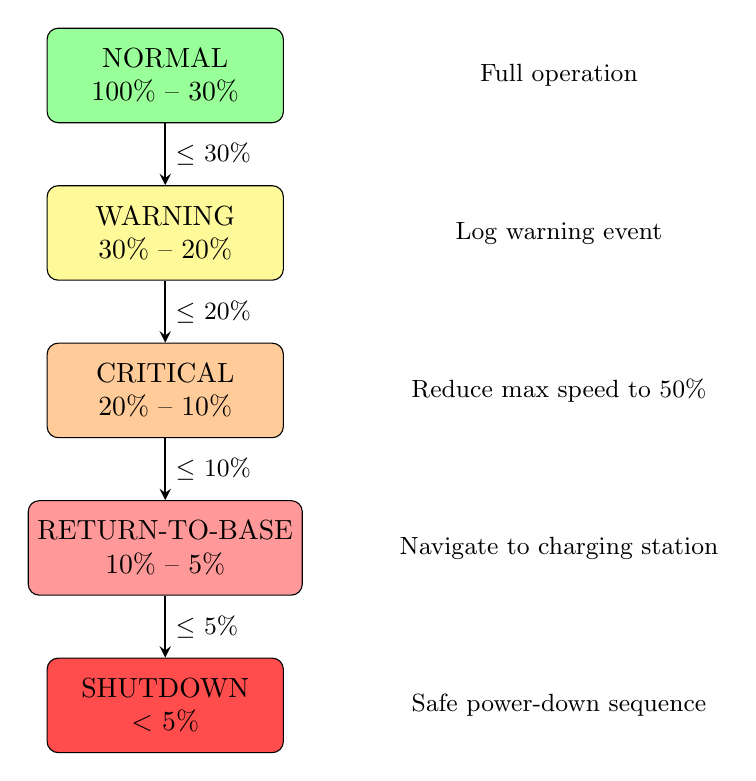
\begin{tikzpicture}[
    state/.style={draw, rectangle, rounded corners, minimum width=3cm, minimum height=1.2cm, align=center},
    arrow/.style={->, thick, >=stealth}
]
    % States arranged vertically
    \node[state, fill=green!40] (normal) at (0,6) {NORMAL\\100\% -- 30\%};
    \node[state, fill=yellow!40] (warning) at (0,4) {WARNING\\30\% -- 20\%};
    \node[state, fill=orange!40] (critical) at (0,2) {CRITICAL\\20\% -- 10\%};
    \node[state, fill=red!40] (rtb) at (0,0) {RETURN-TO-BASE\\10\% -- 5\%};
    \node[state, fill=red!70] (shutdown) at (0,-2) {SHUTDOWN\\$<$ 5\%};

    % Transitions
    \draw[arrow] (normal) -- node[right, font=\small] {$\leq$ 30\%} (warning);
    \draw[arrow] (warning) -- node[right, font=\small] {$\leq$ 20\%} (critical);
    \draw[arrow] (critical) -- node[right, font=\small] {$\leq$ 10\%} (rtb);
    \draw[arrow] (rtb) -- node[right, font=\small] {$\leq$ 5\%} (shutdown);

    % Actions on right side
    \node[align=left, font=\small] at (5,6) {Full operation};
    \node[align=left, font=\small] at (5,4) {Log warning event};
    \node[align=left, font=\small] at (5,2) {Reduce max speed to 50\%};
    \node[align=left, font=\small] at (5,0) {Navigate to charging station};
    \node[align=left, font=\small] at (5,-2) {Safe power-down sequence};

\end{tikzpicture}
\caption{Battery State Machine}
\end{figure}

\begin{table}[H]
\centering
\caption{Battery Management Thresholds}
\begin{tabular}{|c|l|l|}
\hline
\textbf{Level} & \textbf{State} & \textbf{Action} \\
\hline
100\% -- 30\% & Normal & Full operation, no restrictions \\
\hline
30\% & Warning & Log battery warning event to telemetry \\
\hline
20\% & Critical & Reduce maximum speed to 50\% \\
\hline
10\% & Return-to-Base & Abort current task, navigate to charging station \\
\hline
5\% & Emergency & Initiate safe shutdown sequence \\
\hline
\end{tabular}
\end{table}

\subsection{Battery Monitoring}

Battery voltage and state-of-charge are monitored via the ESP32's ADC with filtering:

\begin{lstlisting}[language=C, caption=Battery monitoring (ESP32)]
#include <esp_adc_cal.h>

#define BATTERY_ADC_CHANNEL     ADC1_CHANNEL_6  // GPIO34
#define BATTERY_SAMPLES         16              // Averaging samples
#define VOLTAGE_DIVIDER_RATIO   4.0             // R1=30k, R2=10k
#define BATTERY_MIN_V           10.0            // 3S LiPo empty
#define BATTERY_MAX_V           12.6            // 3S LiPo full

typedef enum {
    BATTERY_NORMAL,
    BATTERY_WARNING,
    BATTERY_CRITICAL,
    BATTERY_RTB,
    BATTERY_SHUTDOWN
} battery_state_t;

static esp_adc_cal_characteristics_t adc_chars;
static battery_state_t current_state = BATTERY_NORMAL;

void battery_init(void) {
    adc1_config_width(ADC_WIDTH_BIT_12);
    adc1_config_channel_atten(BATTERY_ADC_CHANNEL, ADC_ATTEN_DB_11);
    esp_adc_cal_characterize(ADC_UNIT_1, ADC_ATTEN_DB_11,
                             ADC_WIDTH_BIT_12, 1100, &adc_chars);
}

float battery_read_voltage(void) {
    uint32_t adc_sum = 0;

    // Multi-sample averaging for noise reduction
    for (int i = 0; i < BATTERY_SAMPLES; i++) {
        adc_sum += adc1_get_raw(BATTERY_ADC_CHANNEL);
    }
    uint32_t adc_avg = adc_sum / BATTERY_SAMPLES;

    // Convert to voltage
    uint32_t voltage_mv = esp_adc_cal_raw_to_voltage(adc_avg, &adc_chars);

    return (voltage_mv / 1000.0f) * VOLTAGE_DIVIDER_RATIO;
}

uint8_t battery_get_percentage(float voltage) {
    // Linear approximation (for LiPo, use lookup table for accuracy)
    float pct = (voltage - BATTERY_MIN_V) / (BATTERY_MAX_V - BATTERY_MIN_V);
    pct = fmaxf(0.0f, fminf(1.0f, pct));
    return (uint8_t)(pct * 100.0f);
}

battery_state_t battery_update_state(uint8_t percentage) {
    if (percentage <= 5) {
        current_state = BATTERY_SHUTDOWN;
    } else if (percentage <= 10) {
        current_state = BATTERY_RTB;
    } else if (percentage <= 20) {
        current_state = BATTERY_CRITICAL;
    } else if (percentage <= 30) {
        current_state = BATTERY_WARNING;
    } else {
        current_state = BATTERY_NORMAL;
    }
    return current_state;
}
\end{lstlisting}

\subsection{Safe Shutdown Sequence}

When battery reaches critical level (5\%), the system initiates a controlled shutdown:

\begin{enumerate}
    \item \textbf{Stop Motors} -- Immediate motor disable, engage brakes if available
    \item \textbf{Log Position} -- Save current map position to persistent storage
    \item \textbf{Notify User} -- Send critical battery notification via GraphQL subscription
    \item \textbf{Save State} -- Persist navigation state, waypoints, and settings to flash
    \item \textbf{Shutdown Sequence} -- Graceful ROS 2 node shutdown, then Linux poweroff
\end{enumerate}
